\documentclass[uplatex]{jsarticle}
\usepackage{listings}
\lstset{
  basicstyle={\ttfamily},
  identifierstyle={\small},
  commentstyle={\smallitshape},
  keywordstyle={\small\bfseries},
  ndkeywordstyle={\small},
  stringstyle={\small\ttfamily},
  frame={tb},
  breaklines=true,
  columns=[l]{fullflexible},
  numbers=left,
  xrightmargin=0zw,
  xleftmargin=3zw,
  numberstyle={\scriptsize},
  stepnumber=1,
  numbersep=1zw,
  lineskip=-0.5ex
}
\usepackage[dvipdfmx]{graphicx}
\title{画像認識 レポート2}

\author{101730153 佐治 礼仁 saji.ayahito@h.mbox.nagoya-u.ac.jp}
\date{\today}
\begin{document}
\maketitle
\section{色情報を用いた顔検出}
Colabで実装した.
まず,顔画像を読み込み,0.5倍して,画像を表示するソースコードをListing \ref{list:source1}に示し,ソースコードの実行結果を図\ref{fig:result1}に示す.
\begin{lstlisting}[caption=画像読み込みのソースコード,label=list:source1]
import numpy as np
import cv2
import matplotlib.pyplot as plt

from google.colab import files
from google.colab.patches import cv2_imshow

from google.colab import drive

drive.mount('/content/drive/')
%cd "/content/drive/My Drive/Colab Notebooks/"

img=cv2.imread('./images/my-picture.jpg')
height=img.shape[0]#画像サイズ
width=img.shape[1]

SCALE =0.5
imgq=cv2.resize(img,(int(width*SCALE),int(height*SCALE))) #1/10の縮小 (元の画像がおおきいので)
cv2_imshow(imgq)
print (imgq.shape[0])
print (imgq.shape[1])
\end{lstlisting}

\begin{figure}[htbp]
  \begin{center}
    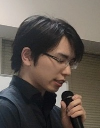
\includegraphics[clip,width=5.0cm]{figures/result1.png}
    \caption{読み込んだ顔画像}
    \label{fig:result1}
  \end{center}
\end{figure}

次に読み込んだ画像をBGR成分からHLS成分へ変更し,色相成分および輝度成分を画像として出力するソースコードをListing \ref{list:source3}に示し,ソースコードの実行結果を図\ref{fig:result3-1},図\ref{fig:result3-2},図\ref{fig:result3-3},図\ref{fig:result3-4}に示す.
\begin{lstlisting}[caption=画像のHLSへの変換,label=list:source3]
imghls=cv2.cvtColor(imgq, cv2.COLOR_BGR2HLS)#BGRからHLS画像への変換
hls = cv2.split(imghls)#HLS画像を各成分に分解

hue = hls[0]#色相画像を使う
cv2_imshow(hue)
hist = cv2.calcHist([hue],[0],None,[256],[0,256])# cv2.calcHist([image], channel, mask, # of bin, range)
print("histgram of hue")
plt.plot(hist) # プロット
plt.xlim([0,256])
plt.show()

lightness = hls[2]#輝度画像を使う
cv2_imshow(lightness)
hist = cv2.calcHist([lightness],[0],None,[256],[0,256])# cv2.calcHist([image], channel, mask, # of bin, range)
print("histgram of lightness")
plt.plot(hist) # プロット
plt.xlim([0,256])
plt.show()
\end{lstlisting}

\begin{figure}[htbp]
  \begin{center}
    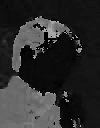
\includegraphics[clip,width=5.0cm]{figures/result3-1.png}
    \caption{顔画像の色相情報の画像化}
    \label{fig:result3-1}
  \end{center}
\end{figure}

\begin{figure}[htbp]
  \begin{center}
    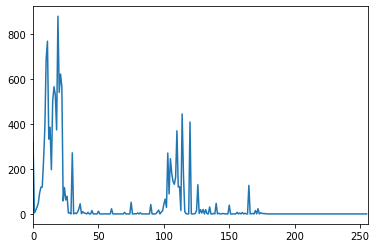
\includegraphics[clip,width=7.5cm]{figures/result3-2.png}
    \caption{顔画像の色相情報のヒストグラム}
    \label{fig:result3-2}
  \end{center}
\end{figure}

\begin{figure}[htbp]
  \begin{center}
    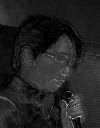
\includegraphics[clip,width=5.0cm]{figures/result3-3.png}
    \caption{顔画像の輝度情報の画像化}
    \label{fig:result3-3}
  \end{center}
\end{figure}

\begin{figure}[htbp]
  \begin{center}
    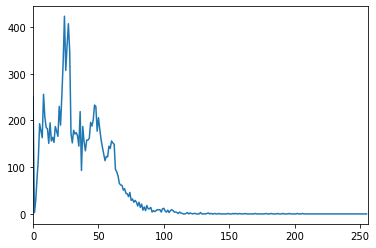
\includegraphics[clip,width=7.5cm]{figures/result3-4.png}
    \caption{顔画像の輝度情報のヒストグラム}
    \label{fig:result3-4}
  \end{center}
\end{figure}


色相情報が10度以上14度以下の制限を用いて顔検出を行うソースコードをListing \ref{list:source4}に示し,ソースコードの実行結果を図\ref{fig:result4}に示す.
この画像に対して,10度以上14度以下と制限を設定することで一番綺麗に顔を検出することができた.
\begin{lstlisting}[caption=色相による顔検出,label=list:source4]
MAX=14#肌色の範囲 14x2=28°以下
MIN=10#肌色の範囲 10x2=20°以上
MASK=200

chroma_key= np.zeros((imgq.shape[0], imgq.shape[1], 1), np.uint8)# 画像領域の準備
for i in range (imgq.shape[0]):
  for j in range (imgq.shape[1]):
    if (hue[i][j] <= MAX) and (hue[i][j] >= MIN):#MAX〜MINを0それ以外をMASKに2値化
      chroma_key[i][j][0] = MASK
    else:
      chroma_key[i][j][0] = 0

cv2_imshow(chroma_key)
\end{lstlisting}

\begin{figure}[htbp]
  \begin{center}
    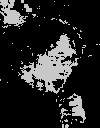
\includegraphics[clip,width=5cm]{figures/result4.png}
    \caption{色相情報による顔検出}
    \label{fig:result4}
  \end{center}
\end{figure}

しかし色相情報だけでは左上部分にノイズが出現しているため,より高い精度で検出するために輝度情報を用いた.
色相情報が10度以上14度以下かつ,輝度情報で48度以上130度以下の制限を用いて顔検出を行うソースコードを\ref{list:source5}に示し,ソースコードの実行結果を図\ref{fig:result5}に示す.
\begin{lstlisting}[caption=色相および輝度による顔検出,label=list:source5]
HUE_MAX=14#肌色の範囲 14x2=28°以下
HUE_MIN=10#肌色の範囲 10x2=20°以上
LIGHTNESS_MAX=130
LIGHTNESS_MIN=48

MASK=200

chroma_key= np.zeros((imgq.shape[0], imgq.shape[1], 1), np.uint8)# 画像領域の準備
for i in range (imgq.shape[0]):
  for j in range (imgq.shape[1]):
    if (hue[i][j] <= HUE_MAX) and (hue[i][j] >= HUE_MIN) and (lightness[i][j] <= LIGHTNESS_MAX) and (lightness[i][j] >= LIGHTNESS_MIN):#MAX〜MINを0それ以外をMASKに2値化
      chroma_key[i][j][0] = MASK
    else:
      chroma_key[i][j][0] = 0

cv2_imshow(chroma_key)
\end{lstlisting}

\begin{figure}[htbp]
  \begin{center}
    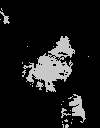
\includegraphics[clip,width=5cm]{figures/result5.png}
    \caption{色相情報による顔検出}
    \label{fig:result5}
  \end{center}
\end{figure}
これによって,色相情報に比べてより制度が高く顔を検出された.以上のコードで正しく顔の検出を行うことができた.

顔以外の部分が検出されてしまうことについて,今回肌色に近い色の座標で検出を行ったため,顔と似た色の壁なども検出されてしまった.
加えて,手は顔と同じ肌色であるため検出されてしまっている.
また,光源の当たり方などで顔の肌色は変わってしまうため,汎用的に適切に顔が検出されるとは言い難く,肌色も人種によって大きく異なるため,さらに汎用的に顔を検出する方法が必要とされると考えた.

\end{document}
